\documentclass[]{article}
\usepackage{ctex,hyperref}% 输出汉字
\usepackage{amsmath,amssymb,amsfonts}
\usepackage{amsthm,amsmath,amssymb}
\usepackage{mathrsfs}
%opening
\usepackage{setspace}
\usepackage{lipsum}
\usepackage{graphicx}% 图片插入宏包
\usepackage{subfigure}% 并排子图
\usepackage{float}% 浮动环境,用于调整图片位置
\usepackage[export]{adjustbox}% 防止过宽的图片
\usepackage{amsmath}
\usepackage{extarrows}
\graphicspath{{Figures/}}%文章所用图片在当前目录下的 Figures目录
\title{波包}
\author{步允霆}

\begin{document}
	
	\maketitle
\section{自由粒子}
若一个粒子在空间各点的势能都为零,我们说它是自由的。\par 
当$V(\mathbf{r},t)=0$,此时的薛定谔方程为
\begin{equation}
	i\hbar\dfrac{\partial}{\partial t}\psi(\mathbf{r},t)=-\dfrac{\hbar^2}{2m}\nabla^2\psi(\mathbf{r},t)
\end{equation}
显然,这个微分方程具有如下形式的解
\begin{equation}
	\psi(\mathbf{r},t)=Ae^{i(\mathbf{k\cdot r}-\omega t)}
\end{equation}
而
\begin{equation}
	\omega=\dfrac{\hbar\mathbf{k}}{2m}
\end{equation}
我们可以看到
\begin{equation}
	|\psi(\mathbf{r},t)|^2=|A|^2
\end{equation}
所以一个这种类型的平面波代表一个粒子,它在空间各点出现的概率是一样的。\par 
根据叠加原理,可以得到
\begin{equation}
	\psi(\mathbf{r},t)=\dfrac{1}{(2\pi)^{3/2}}\int g(\mathbf{k})e^{i[\mathbf{k\cdot r}-\omega (k)t]}\mathrm{d}k
\end{equation}

形如式(5)的波函数,即平面波的叠加,叫做一个三维波包。我们接下来研究平行于Ox轴传播的一维波包,即
\begin{equation}
	\psi(x,t)=\dfrac{1}{\sqrt{2\pi}}\int^{+\infty}_{-\infty} g(k)e^{i[kx-\omega (k)t]}\mathrm{d}k
\end{equation}
若将这个时刻选为时间的起点,则波函数为:
\begin{equation}
	\psi(x,0)=\dfrac{1}{\sqrt{2\pi}}\int g(k)e^{ikx}\mathrm{d}k
\end{equation}
$g(k)$其实就是$\psi(x,0)$的傅里叶变换,即
\begin{equation}
	g(k)=\dfrac{1}{\sqrt{2\pi}}\int \psi(x,0)e^{-ikx}\mathrm{d}x
\end{equation}
因而,式(7)的适用范围并不限于自由粒子。
\section{波包在指定时刻的形状}
假设图1是g(k)的形状,该曲线有一个明显的高峰,极大值位于$k=k_0$处,它的半高处的宽度为$\Delta k$。
\begin{figure}[H]
	\centering
	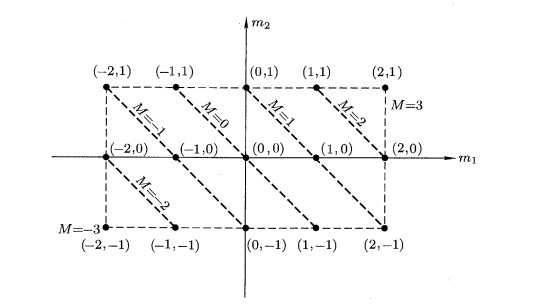
\includegraphics[scale=0.3]{1.png}
	\caption{函数$|g(k)|$的形状}
	\label{Figure 1}
\end{figure}

先考虑一个简单的特例。假设$\psi(x,0)$是三个平面波之和,波矢为$k_0,k_0-\frac{\Delta k}{2},k_0+\frac{\Delta k}{2}$,振幅为0,0.5,0.5。于是我们有:
\begin{align}
	\psi(x)
	&=\dfrac{g(k_0)}{\sqrt{2\pi}}\left[ e^{ik_0x}+\dfrac{1}{2}e^{i(k_0-\Delta k/2)x}+\dfrac{1}{2}e^{i(k_0+\Delta k/2)x}\right] \nonumber\\
	&=\dfrac{g(k_0)}{\sqrt{2\pi}}e^{ik_0x}\left[ 1+\mathrm{cos}\left( \dfrac{\Delta k}{2}x\right) \right] 
\end{align}
容易看出,在x=0处$|\psi(x)|$有极大值。造成这个结果的原因是如下事实:当x取此值的时候,三个波是同相位的,因而他们的干涉是相长的,如图2所示。在x逐渐偏离0以后,三个波的相位便有差异,于是$|\psi(x)|$便减小了。当$e^{ik_0x}$和$e^{i(k_0\pm\Delta k/2)x}$之间的相位差等于$+\pi$时,他们的干涉便是完全相消的;当$x=\pm\Delta x/2$时,$\psi(x)$等于零,$\Delta x$由
\begin{equation}
	\Delta x\cdot\Delta k=4\pi
\end{equation}
给出。此式表示,函数$|g(k)|$的宽度$\Delta k$越小,函数$|\psi(x)|$的宽度$\Delta x$(即$|\psi(x)|$的两个零点间的距离)就越大。
\begin{figure}[H]
	\centering
	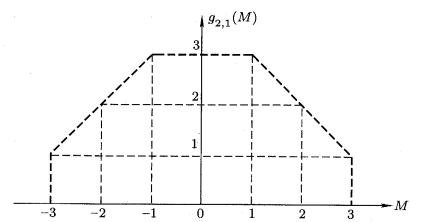
\includegraphics[scale=0.3]{2.png}
	\caption{三个波的实部}
	\label{Figure 2}
\end{figure}

事实上,假设函数$g(k)$的辐角为$\alpha(k)$,即
\begin{equation}
	g(k)=|g(k)|e^{i\alpha(k)}
\end{equation}
如果在$|\psi(x)|$有明显值的区间$\left[ k_0-\dfrac{\Delta k}{2},k_0+\dfrac{\Delta k}{2}\right] $上,$\alpha(k)$的变化是充分正规的,则当$\Delta k$充分小时,我们可在$k=k_0$附近展开$\alpha(K)$
\begin{equation}
	\alpha(k)\simeq\alpha(k_0)+(k-k_0)\left[ \dfrac{\mathrm{d}\alpha}{\mathrm{d}k}\right] _{k=k_0}
\end{equation}
利用此式,可将式(7)重写为
\begin{equation}
	\psi(x,0)\simeq\dfrac{e^{i[k_0x+\alpha(k_0)]}}{\sqrt{2\pi}}\int^{+\infty}_{-\infty} |g(k)|e^{i(k-k_0)(x-x_0)}\mathrm{d}k
\end{equation}
其中
\begin{equation}
	x_0=-\left[ \dfrac{\mathrm{d}\alpha}{\mathrm{d}k}\right] _{k=k_0}
\end{equation}

用式(13)研究$|\psi(x,0)|$随x的变化:当$|x-x_0|$很大时,积分号下k的函数在区间$\Delta k$中有很多次摆动,于是相继各次摆动对积分的贡献互相抵消而使对k积分的结果可以忽略,也就是在远离$x_0$的固定点x处,构成$\psi(x,0)$的各平面波的相位在$\Delta k$的范围内变化得非常迅速,这些波便因干涉而相消,见图3a。反之,若$x\simeq x_0$,则应对k积分的函数实际上并未摆动,因而究$|\psi(x,0)|$有极大值,见图3b。
\begin{figure}[H]
	\centering
	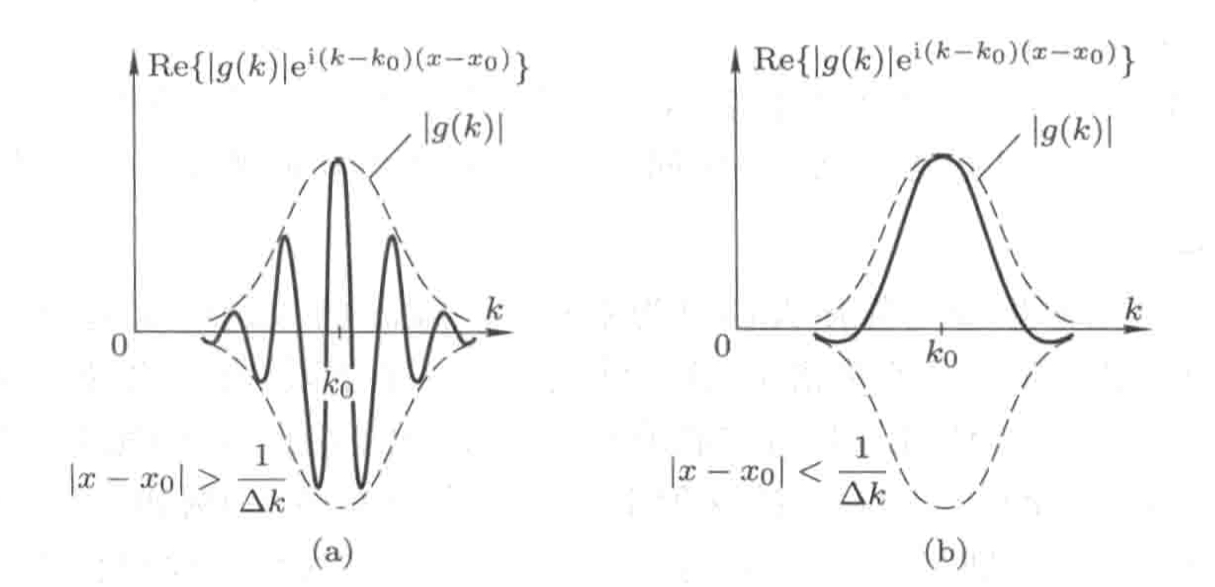
\includegraphics[scale=0.3]{3.png}
	\caption{为了得到$\psi(x,0)$而需对k积分的那个函数随k变化的情况}
	\label{Figure 3}
\end{figure}

于是波包中心的位置为
\begin{equation}
	x_M(0)=x_0=-\left[ \dfrac{\mathrm{d}\alpha}{\mathrm{d}k}\right] _{k=k_0}
\end{equation}

如果振幅最大的那些波,也就是和$k_0$附近的k值对应的那些波,是相长干涉的话,那么像公式(7)中的那种积分将有极大值。相长干涉发生于下述情况:这些波的依赖于k的相位在$k=k_0$附近实际上没有变化。为了得到波包的中心,我们可以认为,相位在k的导数在$k=k_0$处等于零(稳定相位条件)。在上述特例中,和k对应的波的相位是$kx+\alpha(k)$,使得导数$x+\frac{\mathrm{d}\alpha}{\mathrm{d}k}$在$k=k_0$处等于零的x值就是$x_M(0)$\par 
当x偏离$x_0$时,$|\psi(x,0)|$减小;在下述情况下,这种减小更加显著,这种情况是:当k取遍区间$\Delta k$中的值时函数$e^{i(k-k_0)(x-x_0)}$大约摆动一次,这种情况对应于
\begin{equation}
	\Delta k\cdot(x-x_0)\simeq 1
\end{equation}
如果波包的宽度近似地为$\Delta x$,便有
\begin{equation}
	\Delta k\cdot\Delta x\gtrsim 1
\end{equation}
下界的精准值依赖于宽度$\Delta x$和$\Delta k$的定义。\par 
因而,式(6)中的波包表示一个粒子的这样一个态:在时刻t=0,在以$x_0$为中心,近似宽度为$\Delta x$的区间外,该粒子出现的概率实际上为0。
\section{海森伯不确定性}
与一个平面波$e^{i(k-k_0)(x-x_0)}$对应的概率密度在任何时刻t在Ox轴上各点是恒定的,我们可以这样解释:譬如说,在t=0时由$\psi(x,0)=Ae^{ikx}$描述的一个粒子具有完全确定的动量,就是说,在这个时刻去测量他的动量一定得到$p=\hbar k$。由此可见,$e^{ikx}$描述对应于$p=\hbar k$的本征态;另一方面,对k的每一个实数值都存在一个波函数,因此,对于任意态下的一次动量测量,我们预期得到的本征值应包括所有实数值。\par 
现在来研究式(7),在该式中,$\psi(x,0)$表现为动量本征函数的线性叠加,$e^{ikx}$的系数就是$g(k)$。于是我们自然要将$|g(k)|^2$解释为:在时刻t=0测量$\psi(x,t)$所描述的粒子的动量,得到的结果为$p=\hbar k$的概率。但是,实际上p的可能值像x的可能值一样,组成一个连续的数集,而$|g(k)|^2$则正比于一种概率密度:测得p的数值介于$\hbar k$和$\hbar(k+\mathrm{d}k)$之间的概率$\overline{\mathrm{d}\mathscr{P}}$,除去常因子不计时,就是$|g(k)|^2$。更准确地说,如果(7)改写为
\begin{equation}
	\psi(x,0)=\dfrac{1}{\sqrt{2\pi\hbar}}\int\overline{\psi}(p)e^{ipx/\hbar}\mathrm{d}p
\end{equation}
我们就知道,$\overline{\psi}(p)$和$\psi(x,0)$满足贝塞尔-帕塞瓦尔关系式
\begin{equation}
	\int^{+\infty}_{-\infty}|\psi(x,0)|^2\mathrm{d}x=\int^{+\infty}_{-\infty}|\overline{\psi}(x,0)|^2\mathrm{d}p
\end{equation}
将这两个积分的值记作C,那么$\mathrm{d}\mathscr{P}(x)=\dfrac{1}{C}|\psi(x,0)|^2\mathrm{d}x$就是在t=0时,在$x$和$x+\mathrm{d}x$之间找到粒子的概率;同样
\begin{equation}
	\overline{\mathrm{d}\mathscr{P}}(p)=\dfrac{1}{C}|\overline{\psi}(p)|^2\mathrm{d}p
\end{equation}
就是测量动量得到的结果介于$p$和$p+\mathrm{d}p$之间的概率。\par 
回到式(17),我们可以把他写成
\begin{equation}
	\Delta x\cdot\Delta p\geqslant\hbar
\end{equation}
($\Delta p=\hbar\cdot\Delta k$是表示$|\overline{\psi}(p)|$的曲线的宽度)。我们来考虑一个其状态由波包式(18)所确定的粒子;我们知道,在t=0时这个粒子的位置概率仅在$x_0$附近宽度为$\Delta x$的区间内才有显著的值,这就意味着,我们知道的位置带有不确定度$\Delta x$。如果我们在同一时刻测量该粒子的动量,则可能得到介于$p_0+1/2\Delta p$与$p_0-1/2\Delta p$之间的一个数值,这是因为在此区间之外,$|\overline{\psi}(p)|^2$实际上等于零,于是动量的不确定度$\Delta p$,因而对式(21)的解释如下:在任一指定时刻,要以任意高的精准度同时确定粒子的位置和动量是不可能的;当达到(21)所规定的下限时,提高位置的精准度就意味着降低动量的精准度,反之亦然。
\section{自由波包随时间的演变}
我们还是回到一个由一维波包(6)描述的自由粒子。\par 
沿Ox轴传播的某一平面波$e^{i(kx-\omega t)}$的速度为
\begin{equation}
	V_{\varphi}(k)=\dfrac{\omega}{k}
\end{equation}
这是因为平面波只能通过宗量$(x-\dfrac{\omega}{k}t)$而依赖于x和k;$V_{\varphi}(k)$叫做平面波的相速度。带入(3)
\begin{equation}
	V_{\varphi}(k)=\dfrac{\hbar k}{2m}
\end{equation}
我们将会看到,当不同的波具有不同的相速度时,与我们可能预测的相反,波包的极大值位置$x_M$移动的速度并不是平均相速度$\tfrac{\omega}{k}=\tfrac{\hbar k}{2m}$。\par 
回到之前讲的三个波的叠加。对于任意的,$\psi(x,t)$应由下式给出
\begin{align}
	\psi(x,t)
	&=\dfrac{g(k_0)}{\sqrt{2\pi}}\left\lbrace e^{i[k_0x-\omega_0t]}+\dfrac{1}{2}e^{i[(k_0-\Delta k/2)x-(\omega_0-\Delta\omega/2)t]}\nonumber\right.\\
	&\left.\quad+\dfrac{1}{2}e^{i[(k_0+\Delta k/2)x-(\omega_0+\Delta\omega/2)t]}\right\rbrace \nonumber\\
	&=\dfrac{g(k_0)}{\sqrt{2\pi}}e^{i(k_0x-\omega_0t)}\left[ 1+\mathrm{cos}\left( \dfrac{\Delta k}{2}x-\dfrac{\Delta\omega}{2}t\right)  \right] 
\end{align}
于是我们看到,$|\psi(x,t)|$的极大值在t=0时位于x=0处。而现在则位于
\begin{equation}
	x_M(t)=\dfrac{\Delta\omega}{\Delta k}t
\end{equation}
处,而不是在$x_0=\dfrac{\omega_0}{k_0}t$处。这个结果如图4.其中a表示三个波的实部的三个相邻的极大值(1),(2),(3)在t=0时的位置;编号(2)的三个极大值在x=0处重叠,于是在这一点发生相长干涉,这一点就是$|\psi(x,0)|$的极大值的位置。因为相速度随k的增大而增大(式(23)),所以波数为$(k_0+\Delta k/2)$的那个波的极大值(3)将逐渐赶上波数为($k_0$)的那个波的极大值(3),而后者又逐渐赶上波数$(k_0-\Delta k/2)$的那个波的极大值(3)。到了某个时刻,必须出现图4b所示的情况,这时互相重叠的编号为(3)的三个极大值,重合点就是$|\psi(x,t)|$的极大值的位置$x_M(t)$。在图上可以清楚地看到,$x_M(t)$并不等于$\dfrac{\omega_0}{k_0}t$,并且简单计算一下,又可以得出式(25)。
\begin{figure}[H]
	\centering
	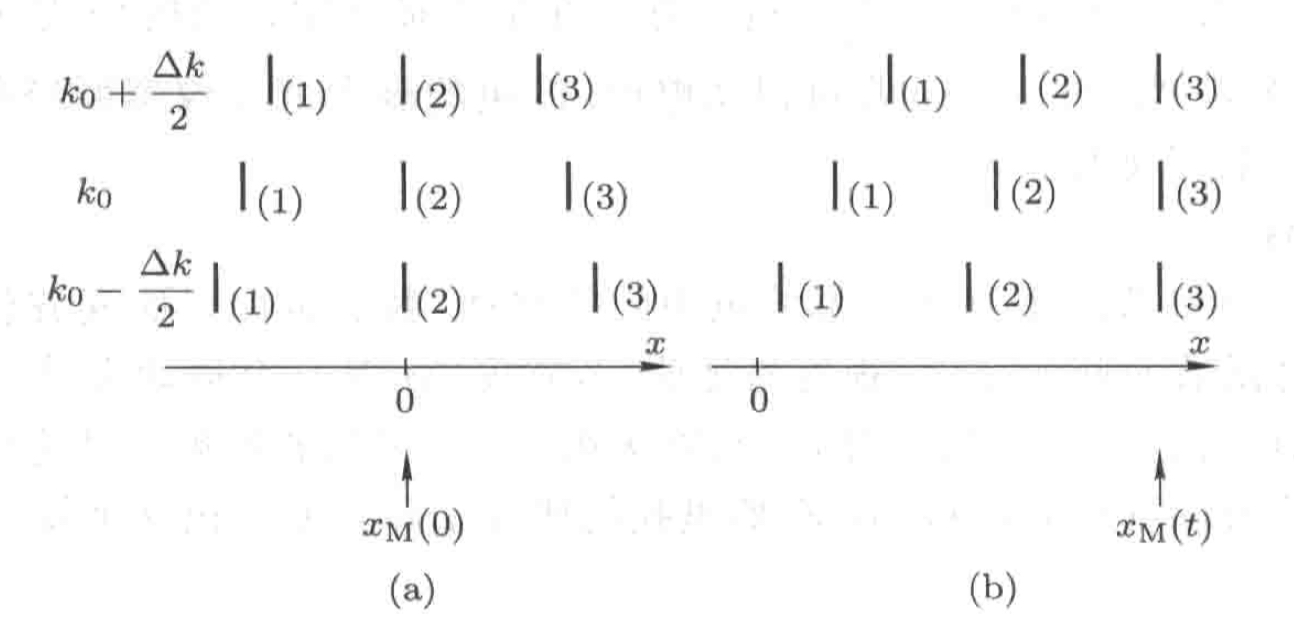
\includegraphics[scale=0.2]{4.png}
	\caption{三个波的极大值的位置}
	\label{Figure 4}
\end{figure}

利用“稳定相位”的方法同样可以求得波包(6)的中心的位移。其实,在自由波包的公式(6)中,我们就可以看出,要从$\psi(x,0)$过渡到$\psi(x,t)$,只需将$g(k)$换成$g(k)e^{-i\omega(k)t}$即可,则辐角为
\begin{equation}
	\alpha(k)-\omega(k)t
\end{equation}
由条件(15)得到
\begin{equation}
	x_M(t)=\left[ \dfrac{\mathrm{d}\omega}{\mathrm{d}k}\right] _{k=k_0}t-\left[ \dfrac{\mathrm{d}\alpha}{\mathrm{d}k}\right] _{k=k_0}
\end{equation}

波包极大值的速度则为
\begin{equation}
	V_G(k_0)=\left[ \dfrac{\mathrm{d}\omega}{\mathrm{d}k}\right] _{k=k_0}
\end{equation}
$V_G(k_0)$叫做波包的群速度。利用色散关系,便可得到
\begin{equation}
	V_G(k_0)=\dfrac{\hbar k_0}{m}=2V_{\varphi}(k_0)
\end{equation}
这个式子也适用于对自由粒子的经典描述。
\section{一维高斯型波包}
\subsection{高斯波包的定义}
在一维模型中,我们考虑一个自由粒子,他的波函数在t=0时的形式为
\begin{equation}
	\psi(x,0)=\dfrac{\sqrt{a}}{(2\pi)^{3/4}}\int^{+\infty}_{-\infty}e^{-\frac{a^2}{4}(k-k_0)^2}e^{ikx}\mathrm{d}k
\end{equation}
这个波包可以由很多像$e^{ikx}$这样的平面波叠加而成,各平面波前面的系数是
\begin{equation}
	\dfrac{1}{\sqrt{2\pi}}g(k,0)=\dfrac{\sqrt{a}}{(2\pi)^{3/4}}e^{-\frac{a^2}{4}(k-k_0)^2}
\end{equation}
这对应于一个中心在$k=k_0$处的高斯函数,因此,我们说(30)的波包是高斯型的。\par 
现在介绍一个实用的积分
\begin{equation}
	\int^{+\infty}_{-\infty}e^{-\alpha^2(\xi+\beta)^2}\mathrm{d}\xi=\dfrac{\sqrt{\pi}}{\alpha}
\end{equation}

现在来计算$\psi(x,0)$。为此,将(30)的指数中含有k的项归并一下,写成下列形式的完全平方
\begin{equation}
	-\dfrac{a^2}{4}(k-k_0)^2+ikx=-\dfrac{a^2}{4}\left[ k-k_0-\dfrac{2ix}{a^2}\right] ^2+ik_0x-\dfrac{x^2}{a^2}
\end{equation}
于是利用(32)算出
\begin{equation}
	\psi(x,0)=\left( \dfrac{2}{\pi a^2}\right) ^{1/4}e^{ik_0x}e^{-x^2/a^2}
\end{equation}
于是我们证明了高斯型函数的傅里叶变换还是高斯型函数。\par
因此,在t=0时,粒子的概率密度由下式给出
\begin{equation}
	|\psi(x,0)|^2=\sqrt{\dfrac{2}{\pi ^2}}\cdot e^{-2x^2/a^2}
\end{equation}

表示$|\psi(x,0)|^2$的曲线就是经典的钟形曲线。波包中心($|\psi(x,0)|^2$的极大值)位于x=0处。
\subsection{不确定度关系式}
研究高斯函数$f(x)=e^{-x^2/b^2}$时,为了方便,将他的宽度明确规定为
\begin{equation}
	\Delta x=\dfrac{b}{\sqrt{2}}
\end{equation}
当x从0变到$\pm\Delta x$的时候,函数的值缩小为原来的$1/\sqrt{e}$;这种规定虽然是任意的,但有一个优点,就是他与变量x的“方均根偏差”一致。\par 
根据这个规定,可以算出(35)中的波包的宽度
\begin{equation}
	\Delta x=\dfrac{a}{2}
\end{equation}

由于$|g(k,0)|^2$也是一个高斯型函数,可以用同样的方法计算他的宽度$\Delta k$,结果得到
\begin{equation}
	\Delta k=\dfrac{1}{a}
\end{equation}
或写作
\begin{equation}
	\Delta p=\dfrac{\hbar}{a}
\end{equation}
从而得到
\begin{equation}
	\Delta x\cdot\Delta p=\dfrac{\hbar}{2}
\end{equation}
这个结果与海森堡不确定性关系完全一致。
\subsection{波包的演变}
\subsubsection{$\psi(x,t)$的计算}
为了计算t时刻的波函数$\psi(x,t)$,只需利用(5),给出自由粒子的波函数,我们得到
\begin{equation}
	\psi(x,t)=\dfrac{\sqrt{a}}{(2\pi)^{3/4}}\int^{+\infty}_{-\infty}e^{-\frac{a^2}{4}(k-k_0)^2}e^{i[kx-\omega(k)t]}\mathrm{d}k
\end{equation}
其中$\omega(k)=\hbar k^2/2m$。我们将会看到,在t时刻,波包仍旧保持为高斯型的。实际上,和前面一样,将指数中含有k的项归并一下,组成完全平方后积分,得
\begin{equation}
	\psi(x,t)=\left( \dfrac{2a^2}{\pi}\right)^{1/4}\dfrac{e^{i\varphi}}{\left( a^4+\dfrac{4\hbar^2t^2}{m^2}\right) ^{1/4}}e^{ik_0x} \mathrm{exp}\left\lbrace -\dfrac{\left[ x-\dfrac{\hbar k_0}{m}t\right] ^2}{a^2+\dfrac{2i\hbar t}{m}}\right\rbrace 
\end{equation}
其中$\varphi$是与x无关的实数
\begin{equation}
	\varphi=-\theta-\dfrac{\hbar k^2_0}{2m}t\quad and \quad \mathrm{tan}2\theta=\dfrac{2\hbar t}{ma^2}
\end{equation}
我们再计算t时刻粒子的概率密度$|\psi(x,t)|^2$,结果为
\begin{equation}
	|\psi(x,t)|^2=\sqrt{\dfrac{2}{\pi a^2}}\dfrac{1}{\sqrt{1+\dfrac{4\hbar^2t^2}{m^2a^4}}}\mathrm{exp}\left\lbrace -\dfrac{2a^2\left( x-\dfrac{\hbar k_0}{m}t\right) ^2}{a^4+\dfrac{4\hbar^2 t^2}{m^2}}\right\rbrace  
\end{equation}

现在证明,波包的模方$\int^{+\infty}_{-\infty}|\psi(x,t)|^2\mathrm{d}x$与时间无关。由(41)可知,$\psi(x,t)$的傅里叶变换就是
\begin{equation}
	g(k,t)=e^{-i\omega(k)t}g(k,0)
\end{equation}
显然,$g(k,t)$与$g(k,0)$具有相同的模方,贝塞尔-帕塞瓦尔等式表明,正如$\psi(x,0)$和$g(k,0)$具有相同的模方一样,$\psi(x,t)$和$g(k,t)$也具有相同的模方。据此便知$\psi(x,t)$和$\psi(x,0)$具有相同的模方。
\subsubsection{波包移动的速度}
从(44)可以看出,概率密度$|\psi(x,t)|^2$也是一个高斯型函数,他的中心在$x=V_0t$处,速度$V_0$由下式给出
\begin{equation}
	V_0=\dfrac{\hbar k_0}{m}
\end{equation}
\subsubsection{波包的扩展}
回到式(44),根据定义(36),波包在t时刻的宽度$\Delta x(t)$应为
\begin{equation}
	\Delta x(t)=\dfrac{a}{2}\sqrt{1+\dfrac{4\hbar^2t^2}{m^2a^4}}
\end{equation}

由此可见(图5),波包的演变并不只是以速率$V_0$移动,他的形状也在变化。当t从$-\infty$增加到0时,波包的宽度不断减小,以致在t=0时减小到最小;然后宽度随t的增大而不断增大(波包在扩展)。\par 
从(44)式还可以看出,波包的高度也在变化,不过与宽度变化的趋势相反,从而使$\psi(x,t)$的模方保持不变。
\begin{figure}[H]
	\centering
	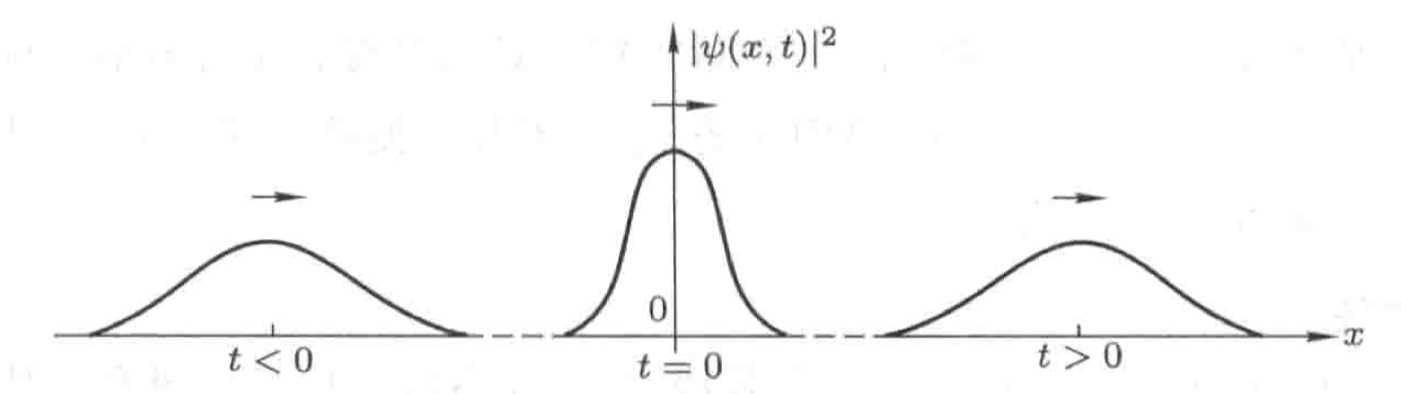
\includegraphics[scale=0.2]{5.png}
	\caption{波包宽度与高度随时间的变化}
	\label{Figure 5}
\end{figure}

函数$g(k,t)$的性质完全不同,因为
\begin{equation}
	|g(k,t)|=|g(k,0)|
\end{equation}
因此,波包的平均动量$(\hbar k_0)$及其动量弥散$(\hbar\Delta k)$都不随时间而变。\par 
由于存在着动量的弥散$\Delta p=\hbar\Delta k=\hbar/a$,确定粒子的速度就只能精确到$\Delta v=\Delta p/m=\hbar/ma$。我们设想一群经典粒子,在t=0时,他们从x=0点出发,速度弥散为$\Delta v$;到了时刻t,这些粒子的位置的弥散将是$\delta x_{cl}=\Delta v|t|=\hbar|t|/ma$;这种弥散是随t线性增大的,如图6。在同一图中,还画出$\Delta x(t)$随时间变化的曲线,当t趋向无穷大时,$\Delta x(t)$与$\delta x_{cl}$实际上是重合的。因此我们说,当t很大时,可以对宽度$\Delta x$作出准经典的解释。反之,t越是接近于0,$\Delta x(t)$的值与$\delta x_{cl}$的值的差别就越大。实际上,一个量子粒子必须时时满足海森堡不确定原理$\Delta x\cdot\Delta p\geqslant\hbar/2$,现在$\Delta p$是固定的,这个不等式便确定了$\Delta x$的下限。
\begin{figure}[H]
	\centering
	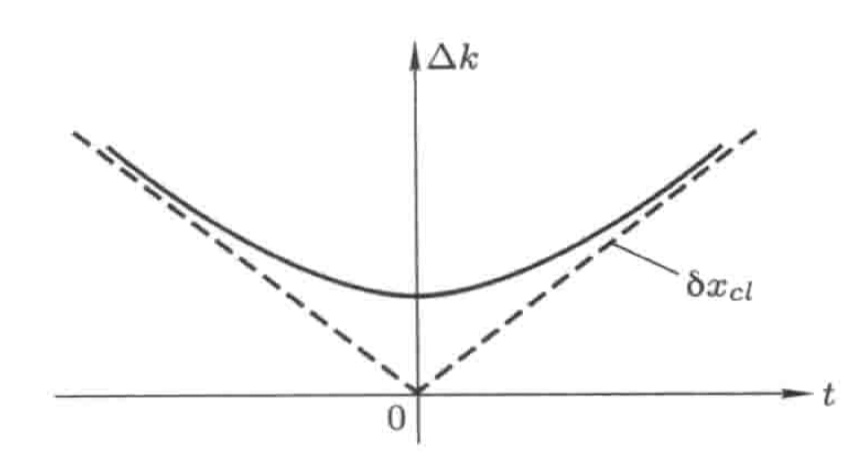
\includegraphics[scale=0.2]{6.png}
	\caption{图5中波包的宽度随时间的变化}
	\label{Figure 6}
\end{figure}
\end{document}